% SOICT 2026 submission - Springer LNCS format (single-blind: keep author names).
% Requires the Springer LNCS class `llncs.cls` + `splncs04.bst`.
% Multi-market volatility forecasting model. Figures in docs/paper/figures/.
% HOSE table (tab:hose) numbers: results/gamma_gbm/full_compare_hose.json (OWN-8, rq dropped, committed).
%   HARQ HOSE row: results/gamma_gbm/paper_metrics_hose.json. GARCH: results/gamma_gbm/garch_hose.json.
% SP500 table (tab:sp500) numbers: results/gamma_gbm/full_compare_sp500.json (OWN-8).
% GNNHAR: results/gamma_gbm/gnnhar_<market>.json. GARCH: results/gamma_gbm/garch_<market>.json.
\documentclass{llncs}
\usepackage{graphicx}
\graphicspath{{figures/}}
\usepackage{booktabs}
\usepackage{amsmath}
\usepackage{amssymb}
\usepackage{placeins}
\usepackage[utf8]{inputenc}
\usepackage[T1,T5]{fontenc}

\begin{document}

\title{Multi-Market Stock Volatility Forecasting Model}

\author{Nguyễn Thành Quy\inst{1} \and Lê Trung Hoàng\inst{1} \and Trần Duy Hoàng\inst{1}}
\institute{University of Science, Vietnam National University Ho Chi Minh City, Ho Chi Minh City, Vietnam \\ \email{lthoang@hcmus.edu.vn}}

\maketitle

\begin{abstract}
Forecasting daily stock-price volatility, how much a stock's price is likely to swing on a given day,
is a core input to risk management and option pricing: a risk manager sizing exposure or a trader
pricing an option needs to know not only which direction a price may move but how large its swings
will be. We propose a per-stock volatility forecasting model built on a gamma-loss gradient-boosting
machine (GBM) over own-history features, and we ask where extra information actually helps. The
own-history GBM already beats the HAR and HARQ linear benchmarks and a per-stock GARCH on QLIKE at
every horizon. On the S\&P~500, adding an External, forward-looking scheduled-earnings feature (GBME)
cuts QLIKE by 8.7 to 11.2\% over own-history at every horizon (Diebold-Mariano $p<0.001$). A learned
graph neural network (GNNHAR) does not beat the own-history GBM on either market. We replicate the
study on a second, structurally different market, 405 Vietnam Ho Chi Minh Stock Exchange (HOSE)
tickers, under an identical leakage-controlled walk-forward protocol scored on QLIKE with
date-clustered Diebold-Mariano tests; the earnings lever does not transfer, which localizes the
earnings gain to the S\&P~500.
\keywords{Volatility forecasting \and HAR \and Gradient boosting \and Earnings announcements \and Diebold-Mariano.}
\end{abstract}

\section{Introduction}
Financial markets are volatile: prices swing, and the size of those swings, an asset's
\emph{volatility}, is the standard measure of its risk. Because volatility drives how options are
priced, how much capital a position ties up, and how risk is budgeted across a portfolio, forecasting
it accurately is a long-standing problem in financial econometrics~\cite{corsi2009}. Volatility is
not observed directly; it is estimated from prices, so any forecast is a forecast of an estimate. We
target the daily \emph{Parkinson estimator}~\cite{parkinson1980}, which gauges a day's variance from
its high-low price range and uses more of the day's information than a close-to-close measure; our
forecasting target is therefore a variance (a squared quantity), not a standard deviation.

The standard linear approach is the HAR family~\cite{corsi2009}: a plain linear regression that
predicts tomorrow's volatility from its own averages over the last day, the last week (about five
trading days), and the last month (about twenty-two), summarising volatility's long memory with a
handful of coefficients. This benchmark is deliberately simple yet hard to beat. We build a stronger
per-stock gradient-boosting model on top of it and ask what extra information actually helps: a
forward-looking, per-firm earnings signal. As a learned-model reference we also train a graph neural
network on the HAR features~\cite{gnnhar2024} and measure it under the same protocol.

We forecast daily Parkinson variance for the S\&P~500 with a per-stock gamma-loss gradient-boosting
model over own-history features, then add a forward-looking earnings feature and measure it under a
leakage-controlled walk-forward protocol scored on QLIKE with date-clustered Diebold-Mariano tests.
The lever that works is forward-looking and specific to the firm. A scheduled earnings release is
known weeks ahead and raises volatility around the announcement~\cite{patell1981}; encoding the distance from the
forecast target to the nearest scheduled release cuts QLIKE by 8.7 to 11.2\% over own-history at
every horizon. A learned graph neural network (GNNHAR), by contrast, does not beat the own-history GBM
on either market.

This paper contributes two results. First, a per-stock gamma-GBM over own-history features is a
strong, transparent baseline for daily volatility that beats HAR, HARQ, a per-stock GARCH, and a
learned graph neural network (GNNHAR) at every horizon. Second, a forward-looking scheduled-earnings
feature is the dominant lever on the S\&P~500, cutting QLIKE by 8.7 to 11.2\% at every horizon
(Diebold-Mariano $p<0.001$); we replicate the study on a second market, 405 Vietnam HOSE tickers,
where the earnings lever does not transfer, which localizes the earnings gain to the S\&P~500.

\paragraph{Terminology.}
\emph{Volatility}: the size of a stock's price fluctuations, the standard proxy for its risk.
\emph{Parkinson estimator}: a day's variance measured from its high-low price range; our forecasting
target is this variance (squared units), not the standard deviation.
\emph{HAR}: a linear model predicting volatility from its own daily, weekly, and monthly averages.
\emph{QLIKE}: a proxy-robust error measure for volatility forecasts that stays reliable when the
target is a noisy proxy~\cite{patton2011}.
\emph{Diebold-Mariano (DM) test}: a test of whether one forecast is more accurate than another by
more than chance, computed from their day-by-day loss differences~\cite{dm1995}.
\emph{Horizon} $h$: how many trading days ahead we forecast ($h\in\{1,5,10,22\}$, roughly a day, week,
fortnight, and month).

\section{Method and Setup}
\textbf{Target and metric.} We forecast daily Parkinson variance
$\mathrm{pk}_t=\ln(H_t/L_t)^2/(4\ln 2)$ from the daily high $H$ and low $L$ ($\ln$ is the natural
logarithm), at horizons $h\in\{1,5,10,22\}$ over 497 S\&P~500 constituents. We report QLIKE as the
primary loss~\cite{patton2011}, alongside MSE, RMSE and MAE. We test significance with a
Diebold-Mariano statistic~\cite{dm1995} on per-trading-date mean loss, with the
Harvey-Leybourne-Newbold small-sample correction~\cite{hln1997}, because within-day stock errors are
dependent.

\textbf{Model.} The forecasting model is a per-stock GBM (a gamma-loss Gradient Boosting
Machine~\cite{friedman2001}: scikit-learn HistGradientBoostingRegressor~\cite{pedregosa2011},
gamma-deviance loss equal to QLIKE up to a constant, 300 iterations, learning rate 0.05, 31 leaves,
L2=1.0, 3-seed ensemble). Its own-history feature vector is $\mathbb{R}^8$: three HAR
lags~\cite{corsi2009} and five log-volatility momentum terms. An
optional External block (GBME) extends it: $\mathbb{R}^4$ of forward-looking scheduled-earnings
features, chiefly the distance from the forecast target to the nearest scheduled release.
Figure~\ref{fig:arch} shows the architecture.

\textbf{Baselines.} HAR~\cite{corsi2009} fits three own-history lags by ordinary least squares. HARQ
adds a realized-quarticity interaction~\cite{harq2016}. GARCH is a per-stock GARCH(1,1) on daily
returns. GNNHAR~\cite{gnnhar2024} is a learned graph neural network (two graph-convolution layers over
the three HAR lags, its best variant). All share the same target, protocol, and positivity floor as
the GBM.

\subsection*{Features}
\textbf{Own-history block (8 features, used by GBM).} Every own-history feature is observable at the
forecast origin $t$. The three HAR lags capture short, medium, and long memory of realized variance
over one day, one trading week ($\mathrm{WK}=5$), and one trading month (22 days):
\begin{align}
\mathrm{har\_daily} = \mathrm{pk}_t, \qquad
\mathrm{har\_weekly} = \frac{1}{5}\sum_{k=0}^{4}\mathrm{pk}_{t-k}, \qquad
\mathrm{har\_monthly} = \frac{1}{22}\sum_{k=0}^{21}\mathrm{pk}_{t-k}.
\end{align}
Five log-volatility momentum terms, built on $\ell_t=\ln(\max(\mathrm{pk}_t,\varepsilon))$ with
$\varepsilon=10^{-8}$, encode recent trend, multi-scale slope, deviation from the recent mean, and a
standardized 22-day level:
\begin{align}
\mathrm{mr\_change} &= \ell_t-\ell_{t-1}, &
\mathrm{mr\_slope5} &= \frac{\ell_t-\ell_{t-5}}{5}, &
\mathrm{mr\_slope10} &= \frac{\ell_t-\ell_{t-10}}{10},\\
\mathrm{mr\_dev5} &= \ell_t-\frac{1}{5}\sum_{k=0}^{4}\ell_{t-k}, &
\mathrm{mr\_z22} &= \frac{\ell_t-\mu_{22}(\ell)}{\sigma_{22}(\ell)+\varepsilon}, &&
\end{align}
where $\mu_{22}$ and $\sigma_{22}$ are the trailing 22-day mean and standard deviation of $\ell$.
Together these summarize the stock's own short-run acceleration and regime level.

\textbf{External earnings block (4 features, used by GBME).} Each earnings feature is evaluated at the
target day $t+h$ from scheduled release dates known weeks ahead, so the block is forward-looking and
leakage-safe. Let $\mathrm{nxt}$ be the trading days from $t+h$ to the next scheduled announcement,
$\mathrm{prv}$ the trading days since the previous one, and $\mathrm{dist}=\min(\mathrm{nxt},\mathrm{prv})$:
\begin{align}
\mathrm{earn\_prox} &= \max\!\Big(0,\,1-\tfrac{\mathrm{dist}}{5}\Big), &
\mathrm{earn\_soon} &= \mathbf{1}[\mathrm{dist}\le 3],\\
\mathrm{earn\_pre} &= \max\!\Big(0,\,1-\tfrac{\mathrm{nxt}}{5}\Big), &
\mathrm{earn\_post} &= \max\!\Big(0,\,1-\tfrac{\mathrm{prv}}{10}\Big).
\end{align}
Here $\mathrm{earn\_prox}$ is a symmetric triangular proximity that peaks at 1 on the announcement day
and reaches 0 once the nearest release is at least a week away, $\mathrm{earn\_soon}$ is a sharp
$\pm 3$-day flag, $\mathrm{earn\_pre}$ rises into the next release, and $\mathrm{earn\_post}$ decays
over a longer 10-day window because post-earnings volatility drift persists longer than the
pre-announcement run-up. Away from any release all four are zero, so GBME reduces to GBM on ordinary
days and activates only in the roughly two-week window around a scheduled release.
Figure~\ref{fig:eventstudy} shows the S\&P~500 median variance rises to about 2.75 times baseline on
the announcement day, which motivates these windows; on HOSE the median stays flat, so the block is
inert there.

\begin{figure}[t]
\centering
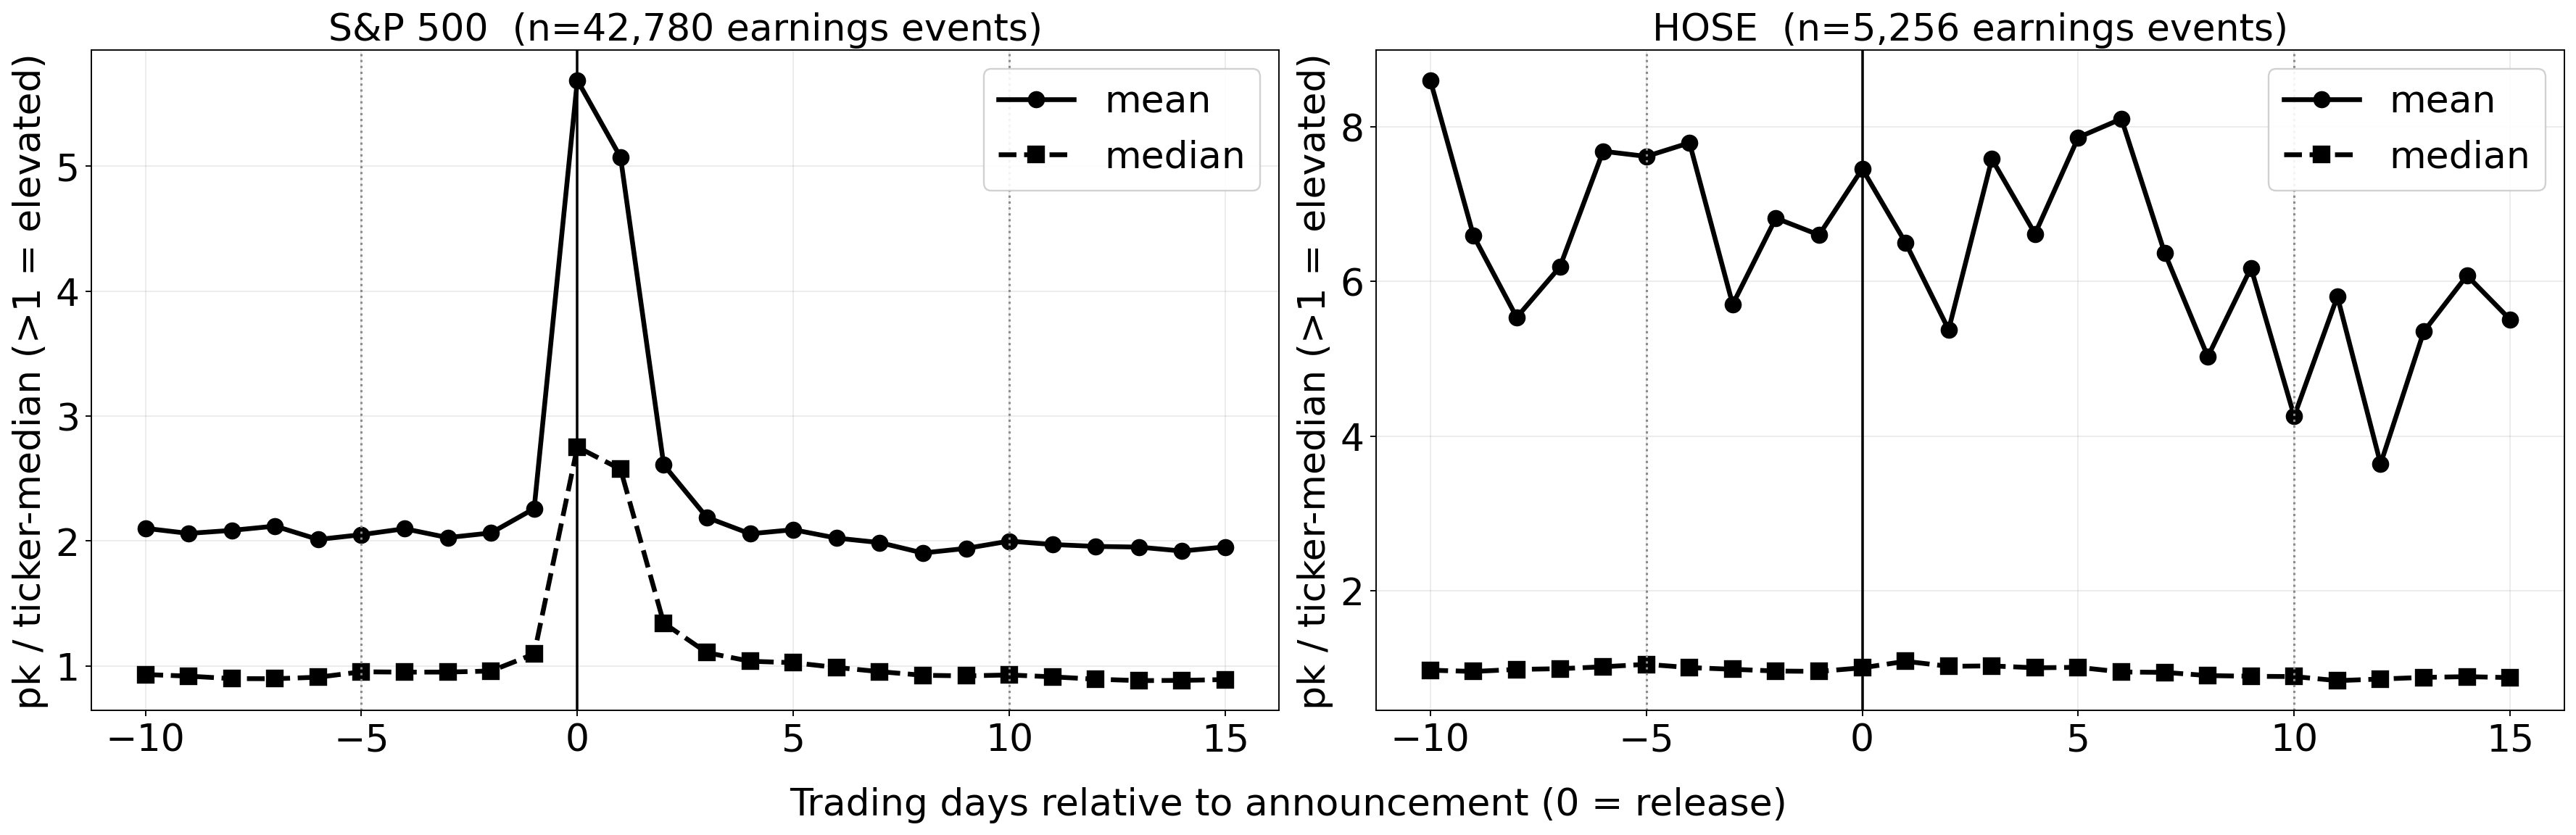
\includegraphics[width=\linewidth]{figures/fig_earnings_event_study.png}
\caption{Event study: median realized Parkinson variance (normalised by each ticker's median) versus
trading days from a scheduled earnings release. The S\&P~500 median rises to about 2.75 times baseline
on the announcement day and returns within roughly a week; the HOSE median stays near one at every
offset, showing no announcement spike, which is why the earnings feature helps the S\&P~500 but not
HOSE.}
\label{fig:eventstudy}
\end{figure}

\textbf{Protocol.} We use expanding-window walk-forward folds with a target-horizon embargo. All
correlations, adjacencies, factor estimates, and model fits use training data only; the test window is
read once. Every gradient-boosting model averages three seeds. Predictions are floored identically
across models before scoring.

\begin{figure}[t]
\centering
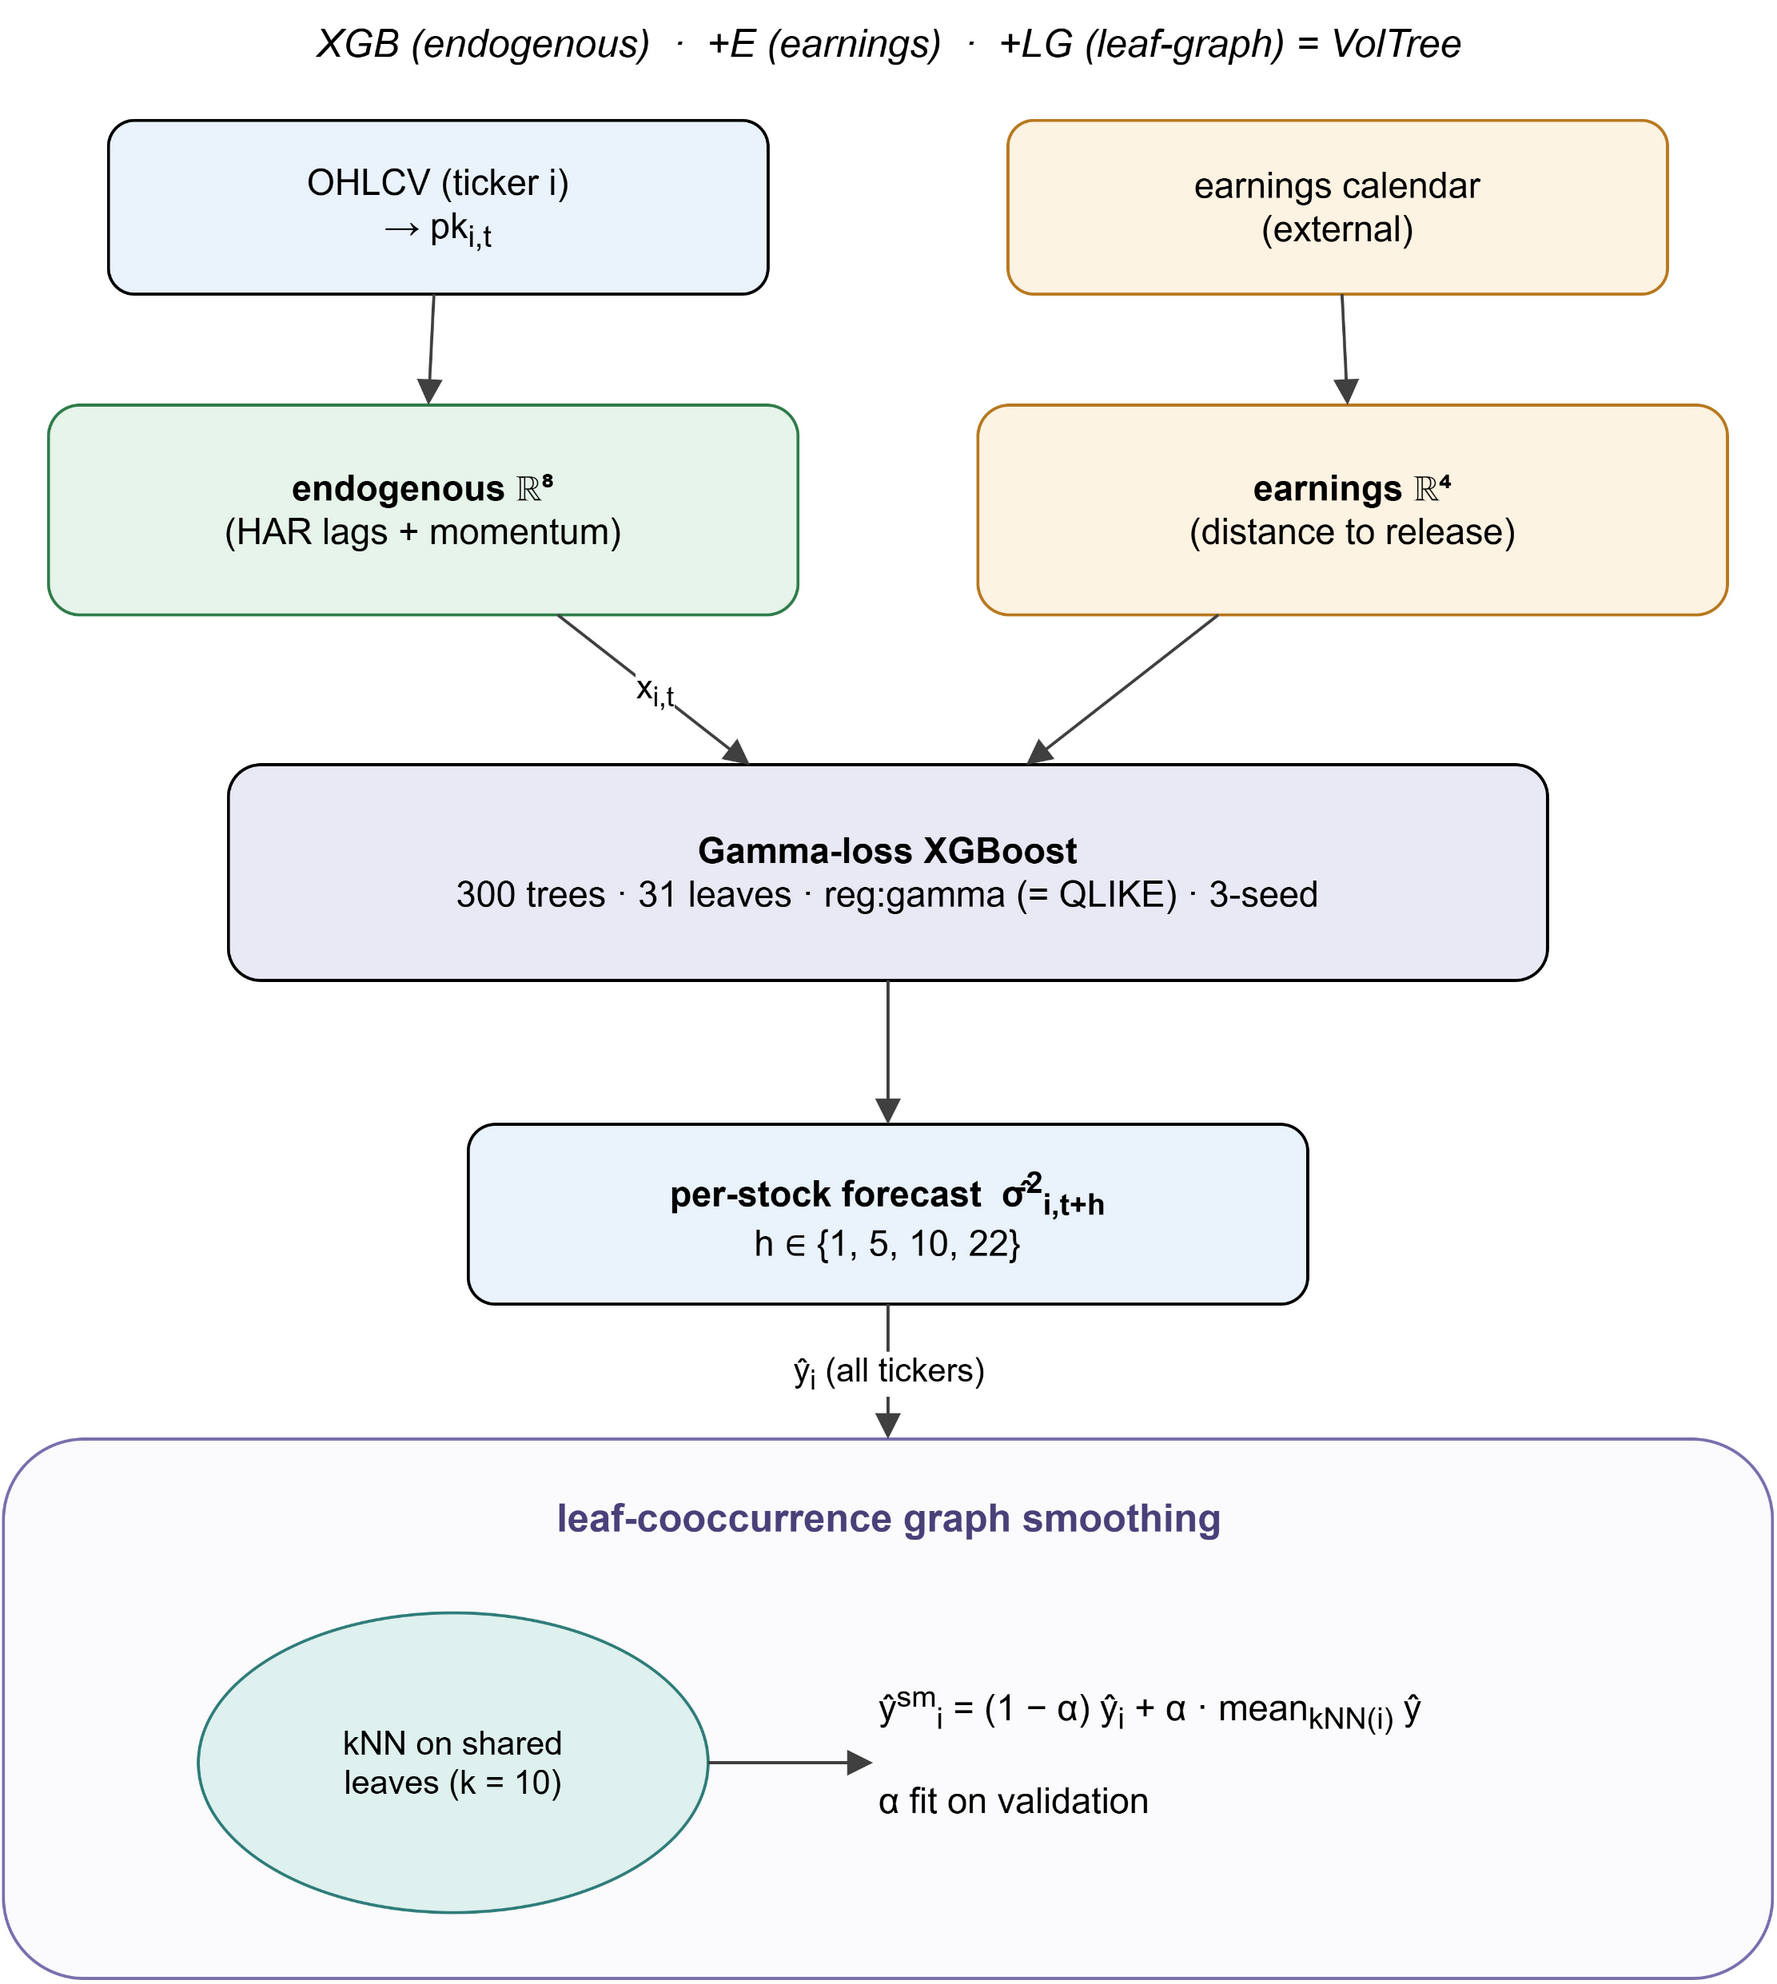
\includegraphics[width=\textwidth]{fig_architecture.png}
\caption{Model architecture. A per-stock feature vector combines own-history features
($\mathbb{R}^8$: three HAR lags and five log-volatility momentum terms) with an optional External
forward-looking scheduled-earnings block ($\mathbb{R}^4$). A gamma-loss gradient-boosting ensemble maps
the feature vector to the multi-horizon Parkinson-variance forecast.}
\label{fig:arch}
\end{figure}

\section{Results: The Own-History GBM Beats the Baselines}\label{sec:graph}
Table~\ref{tab:sp500} reports all four metrics for the S\&P~500 across GARCH, HAR, HARQ, the learned
GNNHAR, the own-history GBM, and the earnings model GBME at every horizon. The own-history GBM beats
HAR, HARQ, and GARCH on QLIKE at every horizon, and the learned GNNHAR does not beat it: GNNHAR is worse than
the GBM at every horizon (QLIKE worse by 5.0 to 10.6\%, DM $p<10^{-10}$) and worse than even linear HAR
at the three shortest horizons, so a multi-hop graph network recovers nothing the own-history GBM does
not already capture. The earnings model GBME carries the bolded QLIKE in every block; the next section
isolates why.

\begin{table}[t]
\centering
\caption{Main result, S\&P~500 (497 constituents; walk-forward, 3-seed ensembles). Lower is better
on every metric. MSE $\times10^{-6}$, RMSE/MAE $\times10^{-3}$; QLIKE unscaled. GARCH is a per-stock
GARCH(1,1) benchmark, QLIKE only; its squared-error cells are shown as \texttt{--}. Bold marks the best
value in each metric column per horizon; the QLIKE bold additionally requires a significant
date-clustered Diebold-Mariano test ($p<0.05$).}
\label{tab:sp500}
\footnotesize
\setlength{\tabcolsep}{6pt}
\begin{tabular}{llcccc}
\toprule
$h$ & Model & MSE & RMSE & MAE & QLIKE \\
\midrule
1 & GARCH       & -- & -- & -- & 0.465 \\
1 & HAR         & 0.575 & 0.759 & 0.213 & 0.370 \\
1 & HARQ        & 0.565 & 0.752 & 0.215 & 0.378 \\
1 & GNNHAR      & 0.576 & 0.759 & 0.212 & 0.375 \\
1 & GBM         & 0.557 & 0.746 & 0.209 & 0.357 \\
1 & GBME        & \textbf{0.540} & \textbf{0.735} & \textbf{0.202} & \textbf{0.317} \\
\midrule
5 & GARCH       & -- & -- & -- & 0.508 \\
5 & HAR         & 0.614 & 0.784 & 0.230 & 0.436 \\
5 & HARQ        & 0.613 & 0.783 & 0.231 & 0.438 \\
5 & GNNHAR      & 0.638 & 0.799 & 0.233 & 0.446 \\
5 & GBM         & 0.611 & 0.782 & 0.226 & 0.412 \\
5 & GBME        & \textbf{0.596} & \textbf{0.772} & \textbf{0.218} & \textbf{0.371} \\
\midrule
10 & GARCH       & -- & -- & -- & 0.522 \\
10 & HAR         & 0.621 & 0.788 & 0.236 & 0.461 \\
10 & HARQ        & 0.621 & 0.788 & 0.236 & 0.461 \\
10 & GNNHAR      & 0.660 & 0.812 & 0.243 & 0.477 \\
10 & GBM         & 0.629 & 0.793 & 0.232 & 0.431 \\
10 & GBME        & \textbf{0.615} & \textbf{0.784} & \textbf{0.225} & \textbf{0.392} \\
\midrule
22 & GARCH       & -- & -- & -- & 0.544 \\
22 & HAR         & 0.633 & 0.795 & 0.242 & 0.485 \\
22 & HARQ        & 0.631 & 0.794 & 0.241 & 0.483 \\
22 & GNNHAR      & 0.635 & 0.797 & 0.241 & 0.476 \\
22 & GBM         & 0.623 & 0.790 & 0.236 & 0.447 \\
22 & GBME        & \textbf{0.609} & \textbf{0.781} & \textbf{0.228} & \textbf{0.408} \\
\bottomrule
\end{tabular}
\end{table}

\FloatBarrier
\section{Forward-Looking Earnings Are the Lever}\label{sec:earn}
\textbf{A diagnostic locates the missing lever.} The own-history GBM beats HAR across the calm
deciles, yet its remaining QLIKE concentrates in the storm decile: decile D9 alone carries 43\% of the
model's total test QLIKE (Fig.~\ref{fig:decile-error}). The model under-forecasts exactly there, where
its median forecast-to-realized ratio falls below one while every calm decile sits above one
(Fig.~\ref{fig:decile-bias}). Permutation importance ranks the three own-history HAR lags far above
every momentum and auxiliary term (Fig.~\ref{fig:importance}), so own-history is exhausted and the
storm component needs a signal from outside the stock's past. A scheduled earnings release is known
weeks ahead and drives the announcement-driven part of these spikes, which makes a forward-looking
earnings feature the natural lever for the residual the GBM cannot reach.

\begin{figure}[t]
\centering
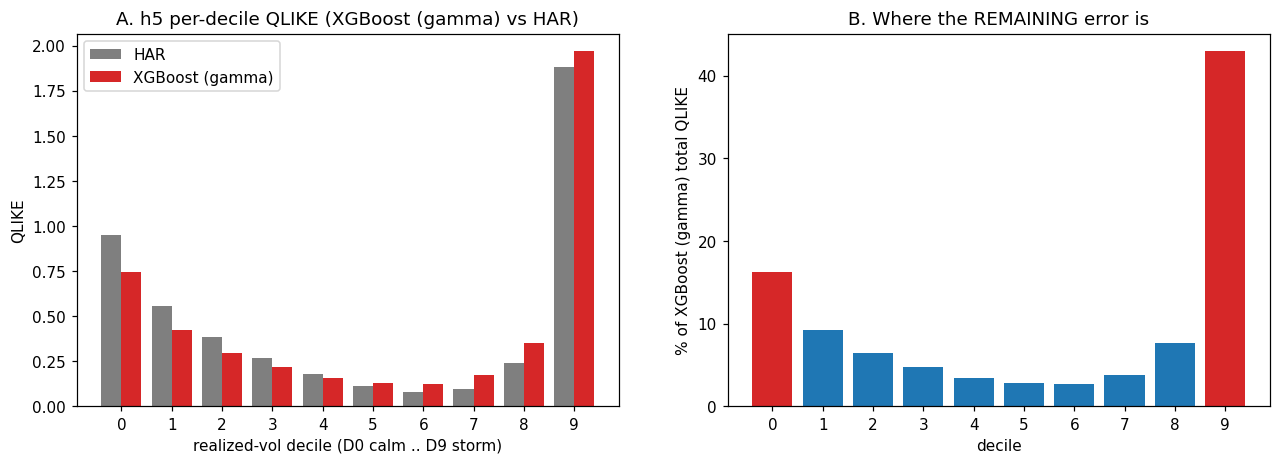
\includegraphics[width=0.85\textwidth]{fig_remaining_error_by_decile.png}
\caption{The own-history GBM beats HAR on the calm deciles, and its remaining QLIKE concentrates in
the storm decile D9, which carries 43\% of the model total.}
\label{fig:decile-error}
\end{figure}

\begin{figure}[t]
\centering
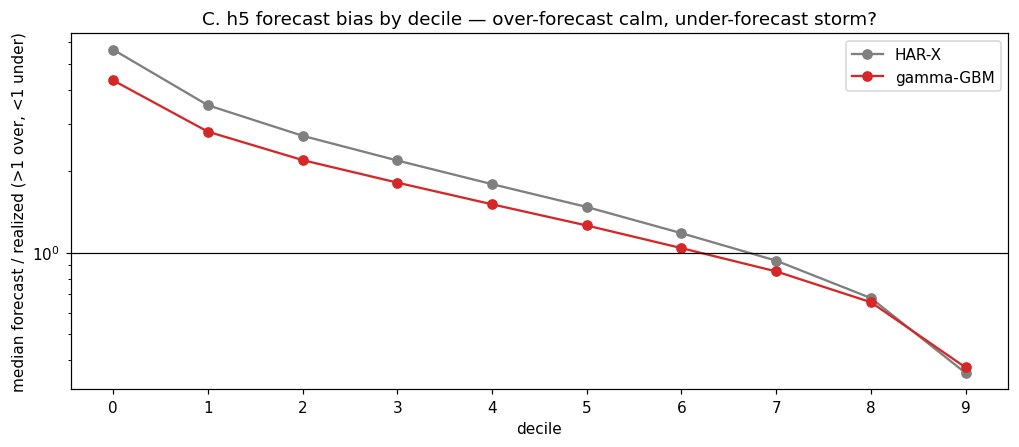
\includegraphics[width=0.85\textwidth]{fig_forecast_bias_by_decile.png}
\caption{The GBM under-forecasts the storm deciles, where its median forecast-to-realized ratio drops
below one.}
\label{fig:decile-bias}
\end{figure}

\begin{figure}[t]
\centering
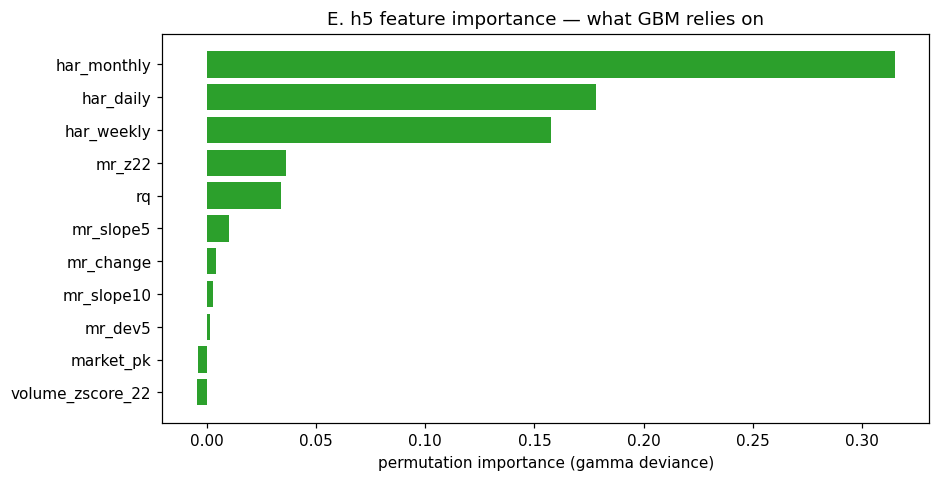
\includegraphics[width=0.85\textwidth]{fig_feature_importance.png}
\caption{Permutation importance ranks the own-history HAR lags far above every other feature, so
own-history is exhausted.}
\label{fig:importance}
\end{figure}

\textbf{The earnings feature is the lever.} In Table~\ref{tab:sp500}, the External earnings model GBME
posts the lowest QLIKE at every horizon. The QLIKE gain over own-history is 8.7 to
11.2\% and is significant at every horizon (DM GBME vs GBM $p<0.001$ at $h1$, $h5$, $h10$, $h22$),
which is why GBME carries the bolded QLIKE in every block. Against the HAR baseline the earnings model
gains 14 to 16\%. Nonlinearity and the QLIKE-loss alignment, isolated by the own-history GBM over HAR,
contribute a further 3.4\%.

\textbf{Earnings do not fix the storm tail.} Decomposed by realized-volatility decile, the model's
error still concentrates in the top decile, which carries roughly ten times the calm-day QLIKE, and
its forecast-to-realized ratio there is about 0.4. The model compresses its predictions toward the
conditional mean because the storm magnitude is absent from origin-time features. The residual is
exogenous, so no origin-time feature reaches it.

\FloatBarrier
\section{Related Work}
\textbf{Neural and graph volatility forecasting.} A recent literature forecasts volatility with graph
neural networks that wire stocks through correlation or spillover edges~\cite{gnnhar2024}. We include the
published GNNHAR as a learned baseline and find, under a leakage-controlled QLIKE walk-forward, that it
does not beat a per-stock gradient-boosting model over own-history features. Prior Vietnamese work builds
correlation and centrality networks to predict index volatility at a monthly horizon without a HAR or
QLIKE benchmark; we extend that setting to daily per-firm QLIKE on 405 HOSE tickers.

\textbf{HAR and its extensions.} HAR~\cite{corsi2009} and HARQ~\cite{harq2016} model volatility from
own history and a realized-quarticity interaction. We keep HAR and HARQ as baselines and show that a
QLIKE-loss gradient-boosting model~\cite{friedman2001,pedregosa2011} with an External earnings feature
dominates them, while QLIKE~\cite{patton2011} and the Diebold-Mariano
test~\cite{dm1995,hln1997} provide the proxy-robust evaluation.

\FloatBarrier
\section{Multi-Market Replication: Vietnam HOSE}\label{sec:hose}
We replicate the study on a second, structurally different market. On 405 Ho Chi Minh Stock Exchange
(HOSE) tickers under the identical protocol, forecasting daily Parkinson variance at the same four
horizons with 390{,}577 to 399{,}040 stock-day observations per horizon, the own-history GBM again wins
and the earnings lever does not transfer.

\textbf{The own-history GBM wins on HOSE too.} Table~\ref{tab:hose} reports all four
metrics. The own-history GBM is the DM-verified best model at every horizon: no feature block
significantly lowers its QLIKE, while HAR and HARQ trail by a wide margin. The External earnings feature
does not improve it: GBME is statistically indistinguishable from GBM at every horizon (DM GBME vs GBM
$p=0.79$, $0.37$, $0.79$, $0.88$ at $h1$, $h5$, $h10$, $h22$). The learned GNNHAR again loses to the GBM
(at $h1$ and $h5$, QLIKE worse by 5.8 to 7.1\%, DM $p<10^{-80}$). The own-history GBM therefore carries
the bolded QLIKE in every block.

\begin{table}[t]
\centering
\caption{Multi-market replication, HOSE (405 tickers; 390{,}577 to 399{,}040 stock-day observations per
horizon). Lower is better on every metric. MSE $\times10^{-6}$, RMSE/MAE $\times10^{-3}$; QLIKE
unscaled. GNNHAR is reported at $h1$ and $h5$. GARCH is a
per-stock GARCH(1,1) benchmark scored on QLIKE over the estimable subset ($\sim$98.6\% of rows); its
squared-error cells are not comparable and shown as \texttt{--}. Bold
marks the best value in each metric column per horizon; the QLIKE bold additionally requires a
significant date-clustered Diebold-Mariano test ($p<0.05$).}
\label{tab:hose}
\footnotesize
\setlength{\tabcolsep}{6pt}
\begin{tabular}{llcccc}
\toprule
$h$ & Model & MSE & RMSE & MAE & QLIKE \\
\midrule
1 & GARCH       & -- & -- & -- & 1.656 \\
1 & HAR         & 0.660 & 0.813 & 0.519 & 1.812 \\
1 & HARQ        & 0.639 & 0.799 & 0.506 & 1.785 \\
1 & GNNHAR      & 0.585 & 0.765 & 0.438 & 1.682 \\
1 & GBM         & \textbf{0.541} & \textbf{0.735} & \textbf{0.394} & \textbf{1.570} \\
1 & GBME        & 0.545 & 0.739 & 0.396 & 1.569 \\
\midrule
5 & GARCH       & -- & -- & -- & 1.740 \\
5 & HAR         & 0.663 & 0.814 & 0.523 & 1.822 \\
5 & HARQ        & 0.652 & 0.807 & 0.515 & 1.807 \\
5 & GNNHAR      & 0.616 & 0.785 & 0.469 & 1.744 \\
5 & GBM         & \textbf{0.579} & \textbf{0.761} & \textbf{0.427} & \textbf{1.648} \\
5 & GBME        & 0.580 & 0.761 & 0.428 & 1.649 \\
\midrule
10 & GARCH       & -- & -- & -- & 1.782 \\
10 & HAR         & 0.666 & 0.816 & 0.525 & 1.828 \\
10 & HARQ        & 0.659 & 0.812 & 0.520 & 1.818 \\
10 & GBM         & \textbf{0.596} & \textbf{0.772} & \textbf{0.442} & \textbf{1.684} \\
10 & GBME        & 0.596 & 0.772 & 0.443 & 1.684 \\
\midrule
22 & GARCH       & -- & -- & -- & 1.837 \\
22 & HAR         & 0.672 & 0.820 & 0.528 & 1.835 \\
22 & HARQ        & 0.668 & 0.817 & 0.525 & 1.830 \\
22 & GBM         & \textbf{0.621} & \textbf{0.788} & \textbf{0.462} & \textbf{1.726} \\
22 & GBME        & 0.623 & 0.789 & 0.462 & 1.726 \\
\bottomrule
\end{tabular}
\end{table}

\textbf{Earnings does not transfer to Vietnam.} Using real crawled Vietnam announcement dates, GBME is
statistically indistinguishable from GBM at every horizon. A per-stock, per-day diagnostic on the HOSE test set
locates two compounding causes. First, the feature fires on only 5.6\% of test observations, and
0.84\% before 2025, so it cannot move the pooled metric across most of the panel. Second, where it
fires the volatility response is muted: realized variance on announcement-proximate days runs about
1.1 times the baseline, against the pronounced S\&P~500 earnings spike, because Vietnam's daily price
limits cap the informational jump. The no-transfer result holds in the well-covered 2025-2026 folds,
so it does not rest on missing dates in that window.

\textbf{The HOSE result is robust to regime spikes.} The own-history GBM beats HAR in every
walk-forward fold (per-fold QLIKE 1.37 to 1.83 against HAR's 1.81 to 1.84), and the margin survives
excluding the COVID (February to April 2020), 2022, and April 2025 tariff shock windows: dropping
those 57{,}466 observations (14\% of the panel) leaves the $h1$ QLIKE gain over HAR at 13.8\% (from
13.3\% on the full panel) and keeps every horizon significant (DM $p<10^{-25}$). The GBM advantage is
a calm-market property, not an artifact of a few crisis days.

\textbf{Takeaway.} The own-history GBM wins on a second, structurally different market. The earnings
lever is specific to the S\&P~500 and does not generalize to HOSE under the available real
announcement dates.

\section{Limitations}
\noindent\textbf{Earnings dates.} The earnings feature measures distance to the nearest scheduled
release from an archive that records realized dates, not a point-in-time scheduling snapshot. A
date-jitter check shows the gain does not depend on exact-date timing: perturbing every S\&P~500
earnings date by a uniform random offset, the $h1$ QLIKE gain over own-history falls from 11.1\% with
true dates to 9.0\% at plus or minus one trading day, 6.6\% at plus or minus three days, and 4.5\% at
plus or minus five days, and stays positive at every horizon. A point-in-time scheduling calendar
remains to be added to control rescheduling within the forecast window.

\noindent\textbf{Vietnam coverage.} The Vietnam earnings test draws on real announcement dates that
are comprehensive only for 2025-01 through 2026-09, plus a sparse 2016-2026 news feed covering roughly
218 tickers. We therefore claim no incremental earnings value on HOSE under the available real dates,
rather than a definitive full-history null.

\noindent\textbf{Scope.} The analysis is conditional on the Parkinson daily-OHLC regime and does not
speak to intraday or option-implied signals.

\section{Conclusion}
We built a per-stock volatility forecasting model on a gamma-loss gradient-boosting machine over
own-history features and asked where extra information helps. The own-history GBM beats the HAR, HARQ,
and GARCH benchmarks and a learned graph neural network (GNNHAR) at every horizon. On the S\&P~500, an
External, forward-looking scheduled-earnings feature cuts QLIKE by 8.7 to 11.2\% at every horizon
(Diebold-Mariano $p<0.001$). We replicated the study on 405 Vietnam HOSE tickers under an identical
protocol: the own-history GBM again wins and the earnings lever does not transfer, which localizes the
earnings gain to the S\&P~500. The practical takeaway is that, for daily volatility, a strong
own-history model plus a forward-looking per-firm signal is what matters, and the value of that signal
depends on the market's information and microstructure.

\begin{thebibliography}{99}
\bibitem{corsi2009} Corsi, F.: A simple approximate long-memory model of realized volatility. J. Financial Econometrics \textbf{7}(2), 174--196 (2009)
\bibitem{parkinson1980} Parkinson, M.: The extreme value method for estimating the variance of the rate of return. J. Business \textbf{53}(1), 61--65 (1980)
\bibitem{harq2016} Bollerslev, T., Patton, A.J., Quaedvlieg, R.: Exploiting the errors: a simple approach for improved volatility forecasting. J. Econometrics \textbf{192}(1), 1--18 (2016)
\bibitem{patton2011} Patton, A.J.: Volatility forecast comparison using imperfect volatility proxies. J. Econometrics \textbf{160}(1), 246--256 (2011)
\bibitem{dm1995} Diebold, F.X., Mariano, R.S.: Comparing predictive accuracy. J. Business \& Economic Statistics \textbf{13}(3), 253--263 (1995)
\bibitem{hln1997} Harvey, D., Leybourne, S., Newbold, P.: Testing the equality of prediction mean squared errors. Int. J. Forecasting \textbf{13}(2), 281--291 (1997)
\bibitem{friedman2001} Friedman, J.H.: Greedy function approximation: a gradient boosting machine. Annals of Statistics \textbf{29}(5), 1189--1232 (2001)
\bibitem{pedregosa2011} Pedregosa, F., et al.: Scikit-learn: machine learning in Python. J. Machine Learning Research \textbf{12}, 2825--2830 (2011)
\bibitem{patell1981} Patell, J.M., Wolfson, M.A.: The ex ante and ex post price effects of quarterly earnings announcements reflected in option and stock prices. J. Accounting Research \textbf{19}(2), 434--458 (1981)
\bibitem{gnnhar2024} Zhang, C., Pu, X., Cucuringu, M., Dong, X.: Graph neural networks for forecasting realized volatility with nonlinear spillover effects. Int. J. Forecasting (2024). arXiv:2308.01419
\end{thebibliography}

\end{document}
